\documentclass[10pt,a4paper]{article}
\usepackage[utf8]{inputenc}
\usepackage[french]{babel}
\usepackage[T1]{fontenc}
\usepackage{amsmath}
\usepackage{amsfonts}
\usepackage{amssymb}
\usepackage{graphicx}
\usepackage{xcolor}

\usepackage{url}
\usepackage{natbib}
\usepackage{fancyhdr}
\usepackage{vmargin}
\usepackage{parskip}

\usepackage{algorithm}
\usepackage{algorithmic}

\usepackage{libertine}
\setlength{\parindent}{0cm}
\setlength{\parskip}{1ex plus 0.5ex minus 0.2ex}
\newcommand{\hsp}{\hspace{20pt}}
\newcommand{\HRule}{\rule{\linewidth}{0.5mm}}

\floatname{algorithm}{Algorithme}
\renewcommand{\algorithmicrequire}{\textbf{Entrée:}}
\renewcommand{\algorithmicensure}{\textbf{Sortie:}}
\renewcommand{\algorithmicif}{\textbf{si}}
\renewcommand{\algorithmicendif}{\textbf{fin si}}
\renewcommand{\algorithmicthen}{\textbf{alors}}
\renewcommand{\algorithmicelse}{\textbf{sinon}}

\begin{document}

\pagestyle{fancy}
\fancyhf{}
\rhead{Salemi Marco, Lecocq Alexis}
\lhead{Priority Search Tree and Windowing}
\cfoot{\thepage}

\begin{titlepage}
  \begin{sffamily}
  \begin{center}

    % Upper part of the page. The '~' is needed because \\
    % only works if a paragraph has started.
    
\includegraphics[scale=0.15]{images/tree.jpg}~\\[1.5cm]

    \textsc{\LARGE U-MONS}\\[2cm]

    \textsc{\Large Rapport de projet de Structures de données 2}\\[1.5cm]

    % Title
    \HRule \\[0.4cm]
    { \huge \bfseries Priority Search Tree and Windowing\\[0.4cm] }

    \HRule \\[2cm]
    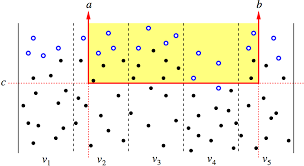
\includegraphics[scale=0.50]{images/window.png}
    \\[2cm]

    % Author and supervisor
    \begin{minipage}{0.4\textwidth}
      \begin{flushleft} \large
        \emph{\textbf{Directeurs :}}\\ BRUYÈRE Véronique \\ DEVILLEZ Gauvain \\
      \end{flushleft}
    \end{minipage}
    \begin{minipage}{0.4\textwidth}
      \begin{flushright} \large
        \emph{\textbf{Groupe :}}\\  SALEMI Marco \\  LECOCQ Alexis
      \end{flushright}
    \end{minipage}

    \vfill

    % Bottom of the page
    {\large \today}

  \end{center}
  \end{sffamily}
\end{titlepage}

\newpage
\tableofcontents
\newpage
\section{Introduction}
Dans le cadre du cours de structures de données 2, nous avons été amenés à réaliser un projet en Java. Ce projet a pour objectif de créer et manipuler une structure de données non vue au cours. Cette nouvelle structure se base sur un arbre de recherche à priorité (Priority Search Tree en anglais ou PST). De la documentation nous a été fournie afin de nous familiariser avec cette dernière structure qui elle non plus n'a pas été vue au cours.

L'objectif du PST est d'appliquer un "windowing" efficace sur un ensemble de données. Le windowing est une technique qui consiste à extraire tous les points qui sont visibles dans une fenêtre donnée. Un exemple pratique et répandu est l'affichage d'une carte sur un GPS : le GPS n'affichera pas toutes les routes qui se trouvent dans le monde mais seulement celles qui nous entourent.

Un PST partage certaines caractéristiques avec les tas et les Arbres Binaires de Recherche ou ABR. Ces deux dernières structures de données ayant été étudiées en profondeur lors des séances de cours, nous les considérons ici comme connues.

\section{Présentation du problème}
Il nous a été demandé d'écrire un programme qui permette d'appliquer un windowing à un ensemble de segments de droite verticaux et horizontaux dans $\mathbb{R}^2$. Les différentes fenêtres à implémenter sont les suivantes :
\begin{itemize}
	\item $[X, X']$ x $[Y, Y']$ ;
	\item $[-\infty, X']$ x $[Y, Y']$ ;
	\item $[X, +\infty]$ x $[Y, Y']$ ;
	\item $[X, X']$ x $[-\infty, Y']$ ;
	\item $[X, X']$ x $[Y, +\infty]$.
\end{itemize}
La structure de données à imaginer devrait donc permettre un windowing efficace pour l'ensemble de ses fenêtres.


\newpage
\section{Priority Search Tree}

\subsection{Objectif de la structure}
Un PST est une structure de données de type arbre binaire (chaque nœud comporte au plus deux fils). Cette structure de données organise des points de l'espace définis par deux coordonnées X et Y. L'organisation des données permet d'effectuer efficacement la recherche des points présents dans une fenêtre de l'espace (sans avoir à parcourir l'ensemble des points).

\subsection{Définition}
Un PST est une structure de données mixte. Chaque nœud est constitué d'un point et d'un nombre appelé la médiane. Si l'on considère uniquement les coordonnées X, un PST est organisé tel un tas avec le minimum à la racine. Si l'on considère uniquement les coordonnées Y, le PST est organisé tel un ABR avec une petite particularité. Au lieu de trier ses fils par rapport à la donnée du nœud courant, un PST trie ses fils par rapport à la médiane du nœud courant.

Ainsi, tout nœud n d'un PST respecte les contraintes suivantes :
\begin{itemize}
	\item son fils gauche (s'il existe, ainsi que ses descendants s'ils existent) aura sa coordonnée X plus grande que celle du nœud n et sa coordonnée Y plus petite que la médiane du nœud n ;
	\item son fils droit (s'il existe, ainsi que ses descendants s'ils existent) aura sa coordonnée X plus grande que celle du nœud n et sa coordonnée Y plus grande que la médiane du nœud n.
\end{itemize}

\subsection{Construction}
Bien que la documentation suggérait une construction bottom-up similaire à celle d'un tas, nous avons opté pour une construction top-down qui nous semblait plus facile à implémenter.

\subsubsection{Tri des données}
La construction d'un PST est plus simple si l'on construit ce dernier à partir d'une liste de points triée selon la coordonnée Y. La première étape est donc de trier les points.

\subsubsection{Création de l'arbre}
Pour créer un arbre, créons le nœud racine à partir de la liste des points triée.

\subsubsection{Création d'un nœud}
La coordonnée X d'un nœud devant être plus petite ou égale à celle de ses fils, commençons par rechercher le point avec la plus petite coordonnée X. Attribuons ce point au nœud courant. Séparons le reste des points en deux. Attribuons, comme médiane au nœud courant, la moyenne de la coordonnée Y de 2 points. Le premier est le dernier point de la partie 1 et le second est le premier point de la partie 2. Les points étant triés selon la coordonnée Y, la première partie possède une coordonnée Y plus petite ou égale à la médiane du nœud alors que la deuxième partie possède une coordonnée Y plus grande ou égale à la médiane du nœud. Dans le cas où il ne reste aucun point après le retrait du minimum en X, la valeur de la moyenne n'a pas d'importance. Dans le cas où il ne reste qu'un point, la coordonnée Y du point restant peut être attribuée à la médiane du nœud.

% TODO insert code

\subsection{Windowing}
L'application du windowing commence à la racine de l'arbre et se déroule comme suit :
\begin{itemize}
	\item si la coordonnée X du nœud courant et strictement supérieure à la borne supérieure de la fenêtre X', alors laisser tomber ce nœud ainsi que tous ses descendants (par définition du PST, leur coordonnée X sera aussi supérieure à X') ;
	\item si le point du nœud courant se trouve dans la fenêtre, le rapporter ;
	\item si la médiane du nœud courant est inférieure ou égale à la borne supérieure de la fenêtre, parcourir le fils gauche ;
	\item si la médiane du nœud courant est supérieure ou égale à la borne inférieure de la fenêtre, parcourir le fils droit ;
\end{itemize}

% TODO insert code

\newpage
\section{PST Adapté}

Étant donné que notre structure utilise des segments au lieu des points, nous ne pouvons utiliser le PST tel que décrit ci-dessus. Nous avons donc adapté cette structure afin de permettre l'utilisation de segments.

Un segment :
\begin{itemize}
	\item est défini par 2 points, chacun ayant une coordonnée X et une coordonnée Y ;
	\item possède donc 2 coordonnées X ainsi que 2 coordonnées Y ;
	\item est soit horizontal soit vertical, c'est-à-dire soit les coordonnées X soit les coordonnées Y sont égales.
\end{itemize}

Nous avons considéré deux façons d'adapter le problème :
\begin{enumerate}
	\item stocker les deux points définissant chaque segment séparément dans la structure initiale, tout en gardant un lien vers le segment initial ;
	\item stocker chaque segment dans une nouvelle structure et adapter les différents algorithmes.
\end{enumerate}

Après mûre réflexion, nous avons opté pour la seconde option, plus flexible et qui nous permet donc davantage d'optimisations.

Afin de garder les explications concises et faciles à comprendre, nous allons d'abord considérer uniquement les fenêtres de type $[X, X']$ x $[Y, Y']$ et $[-\infty, X']$ x $[Y, Y']$ et nous expliquerons ensuite comment gérer les autres cas.

\subsection{Objectif de la structure}
L'objectif de cette structure est d'organiser l'ensemble des segments afin de faciliter la recherche de segments visibles dans les fenêtres de type $[X, X']$ x $[Y, Y']$ et $[-\infty, X']$ x $[Y, Y']$.

\subsection{Définition}
Notre PST adapté respecte exactement la définition d'un PST excepté 2 adaptation :
\begin{itemize}
	\item un segment, plutôt qu'un point, sera stocké par nœud ;
	\item les coordonnées utilisées pour effectuer la comparaison sont le minimum des coordonnées X et le minimum des coordonnées Y du segment, plutôt que les coordonnées X et Y du point.
\end{itemize}

Le choix des coordonnées de référence est judicieux car il permet, lors de la recherche d'une fenêtre, d'élaguer tout nœud (ainsi que ses descendants par définition du tas) dont la coordonnée minimum en X est strictement supérieure à X' et il permet de ne pas visiter le fils droit (ainsi que ses descendants par définition de l'ABR) de tout nœud dont la médiane est strictement supérieure à Y'.

\subsection{Construction}
Notre PST adapté se construit à la manière d'un PST excepté les références pour la comparaison des données, qui sont les coordonnées minimales en X ainsi qu'en Y. C'est-à-dire que nous trions les segments selon leur plus petite coordonnée en Y. Lorsque nous recherchons le minimum en X, nous recherchons le segment avec la plus petite coordonnée X.

\subsection{Windowing}
Étant donné que nous devons rapporter tous les segments visibles dans une certaine fenêtre, nous devons non seulement extraire les segments ayant au moins un point dans la fenêtre, mais aussi les segments commençant avant et finissant après (ceux qui passent à travers la fenêtre). C'est le cas notamment du segment possédant les coordonnées (X', Y-1) (X', Y'+1). La recherche sera donc un peu moins efficace que pour les points et nous allons devoir utiliser une approche différente.

Nouvelle approche : nous concentrer sur le point de départ du segment, c'est-à-dire le point ayant la plus petite coordonnée X pour un segment horizontal ou le point ayant la plus petite coordonnée Y pour un segment vertical. Nous avons ici 3 possibilités pour que le segment soit visible :
\begin{itemize}
	\item soit le point de départ est dans la fenêtre ;
	\item soit le point de départ est à gauche de la fenêtre et le segment traverse la limite gauche de la fenêtre ;
	\item soit le point de départ est en dessous de la fenêtre et le segment traverse la limite basse de la fenêtre.
\end{itemize}
Il est évident que si le point de départ se situe au-dessus ou à droite de la fenêtre, ce segment ne sera pas visible dans la fenêtre.
% TODO add schema of the window to help comprehension

Nous allons donc parcourir l'arbre à partir de la racine et le traiter de la sorte :
\begin{itemize}
	\item si le minimum en X du segment est strictement supérieur à X', laisser tomber ce nœud ainsi que tous ses descendants (le point de départ de leurs segments se situe à droite de la fenêtre) ;
	% TODO add reference to ci-desssus
	\item si ce segment est visible dans la fenêtre (voir conditions ci-dessus), le rapporter ;
	\item si la médiane du nœud est strictement supérieure à Y', laisser tomber le fils droit ainsi que tous ses descendants (le point de départ de leurs segments se situe au dessus de la fenêtre) et parcourir uniquement le fils gauche, sinon parcourir les deux fils.
\end{itemize}
% TODO image de l'arbre et des noeud parcourus

% TODO insert code ?
L'utilisation de cette structure pour réaliser un windowing de type $[-\infty, X']$ x $[Y, Y']$ est très efficace car aucun nœud inutile n'est parcouru.


\subsection{Les autres fenêtres}
Nous avons implémenté un algorithme efficace pour les fenêtres de type $[X, X']$ x $[Y, Y']$ et $[-\infty, X']$ x $[Y, Y']$. Voyons comment l'adapter aux autres fenêtres, à savoir $[X, +\infty]$ x $[Y, Y']$, $[X, X']$ x $[-\infty, Y']$ et $[X, X']$ x $[Y, +\infty]$.

Nous remarquons que 4 des 5 fenêtres partagent une particularité :  elles sont semi-bornées. Nous remarquons également que la place de la borne infinie dépend du système d'axe utilisé. Deux choix sont alors possibles :
\begin{enumerate}
	\item implémenter 3 autres arbres supplémentaires qui sont efficaces pour chacune des autres bornes infinies ;
	\item effectuer une transformation du système d'axe avant la création de l'arbre afin de réutiliser le PST existant.
\end{enumerate}

Maintenir 4 implémentations différentes du PST ne nous a pas semblé être une bonne idée et, la transformation du système d'axe pouvant se faire en temps constant, nous avons opté pour le second choix.

Pour effectuer un windowing avec une fenêtre de type $[X, +\infty]$ x $[Y, Y']$, $[X, X']$ x $[-\infty, Y']$ ou $[X, X']$ x $[Y, +\infty]$, il faudra construire le PST avec les segments transformés dans le nouveau système d'axe, appliquer le windowing sur la fenêtre transformée et appliquer la transformation inverse sur la réponse du windowing.

\subsubsection{L'échange}
Pour passer d'une fenêtre de type $[-\infty, X']$ x $[Y, Y']$ à une fenêtre de type $[X, X']$ x $[-\infty, Y']$, nous remarquons qu'il suffit d'échanger les coordonnées X et Y :
\begin{enumerate}
	\item $X \rightarrow Y$
	\item $Y \rightarrow X$
\end{enumerate}

Nous appellerons cette transformation du système d'axe l'\textbf{échange}.

Nous remarquons qu'effectuer une transformation inverse revient à appliquer la transformation une seconde fois.

\subsubsection{L'opposition}
Pour passer d'une fenêtre de type $[-\infty, X']$ x $[Y, Y']$ à une fenêtre de type $[X, +\infty]$ x $[Y, Y']$, nous remarquons qu'il suffit d'opposer les coordonnées :
\begin{enumerate}
	\item $X \rightarrow -X$
	\item $Y \rightarrow -Y$
\end{enumerate}

Nous appellerons cette transformation du système d'axe l'\textbf{opposition}.

Nous remarquons que, comme pour l'échange, effectuer une transformation inverse revient à appliquer la transformation une seconde fois.

\subsubsection{La combinaison des deux}
Pour passer d'une fenêtre de type $[-\infty, X']$ x $[Y, Y']$ à une fenêtre de type $[X, X']$ x $[Y, +\infty]$, nous remarquons qu'il suffit d'appliquer les deux transformations vues précédemment :
\begin{enumerate}
	\item $X \rightarrow -Y$
	\item $Y \rightarrow -X$
\end{enumerate}

Nous appellerons cette transformation du système d'axe la \textbf{combinaison}.

Encore une fois, effectuer une transformation inverse revient à appliquer la transformation une seconde fois.

\subsubsection{La fenêtre fermée}
Lors de la recherche dans une fenêtre fermée avec le PST original, nous ne pouvons jamais éliminer le fils gauche de nos recherches. En conséquence, les nœuds que nous parcourons, ayant un minimum en X strictement inférieur au X de la fenêtre et ayant un minimum en Y strictement inférieur au Y de la fenêtre, sont parcourus inutilement. Ces segment sont ceux qui commencent en bas à gauche de la fenêtre et il est évident qu'ils n'y sont pas visibles. Nous avons donc adapté notre windowing afin qu'il prenne deux paramètres :
\begin{itemize}
	\item center : définit si les segments commençant au centre de la fenêtre doivent être reportés ;
	\item down : définit si les segments commençant en dessous de la fenêtre doivent être reportés.
\end{itemize}
Si center est faux, alors nous pouvons laisser tomber les nœuds qui ont un minimum en X plus grand que le X de la fenêtre.
Si down est faux, alors nous pouvons laisser tomber les fils gauches des nœuds dont la médiane est strictement inférieure au Y de la fenêtre.

Afin d'effectuer la recherche de la fenêtre fermée efficacement, nous appliquerons le windowing deux fois. Une première fois avec down à faux afin de rapporter les segments ayant le point de départ à gauche et dans la fenêtre. Une seconde fois sur la fenêtre échangée avec la même technique que pour la fenêtre $[X, X']$ x $[-\infty, Y']$ avec center et down à faux afin de rapporter tous les segments ayant leur point de départ en dessous.

\newpage
\section{Diagrammes de classes}
Cette section comporte 2 diagrammes de classes :
\begin{enumerate}
	\item le premier concerne l'organisation et le traitement des données ;
	\item le second concerne l'interface graphique.
\end{enumerate}
Ces diagrammes sont suivis de quelques explications sur les classes implémentées. Si vous désirez de plus amples d'informations, n'hésitez pas à consulter la Javadoc.
% TODO make link to javadoc

\subsection{Diagramme de classe des données}
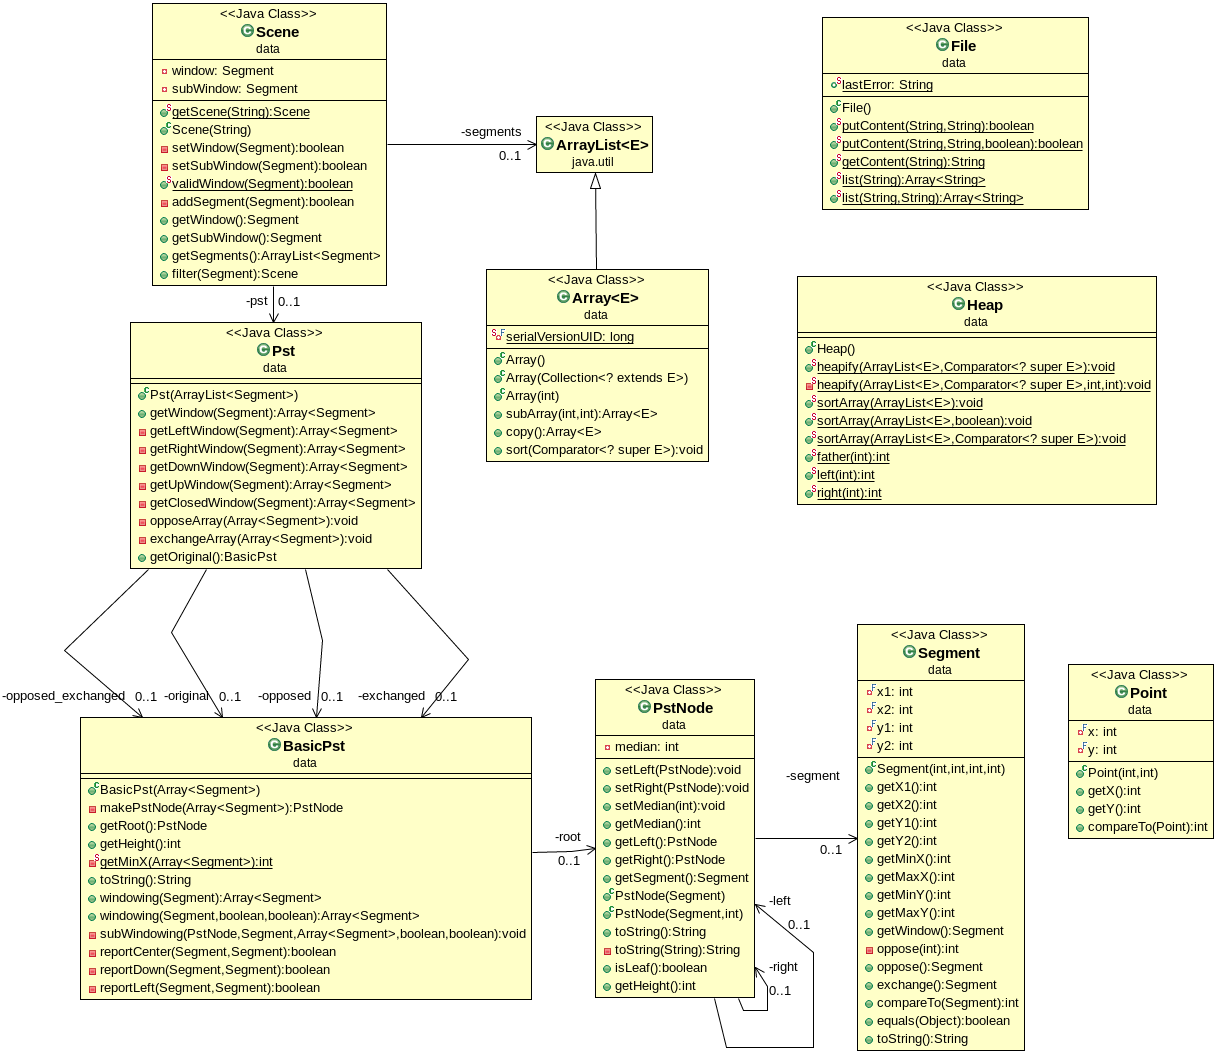
\includegraphics[scale=0.35]{../src/UML/data.png}

\subsection{Diagramme de classe de l'interface graphique}
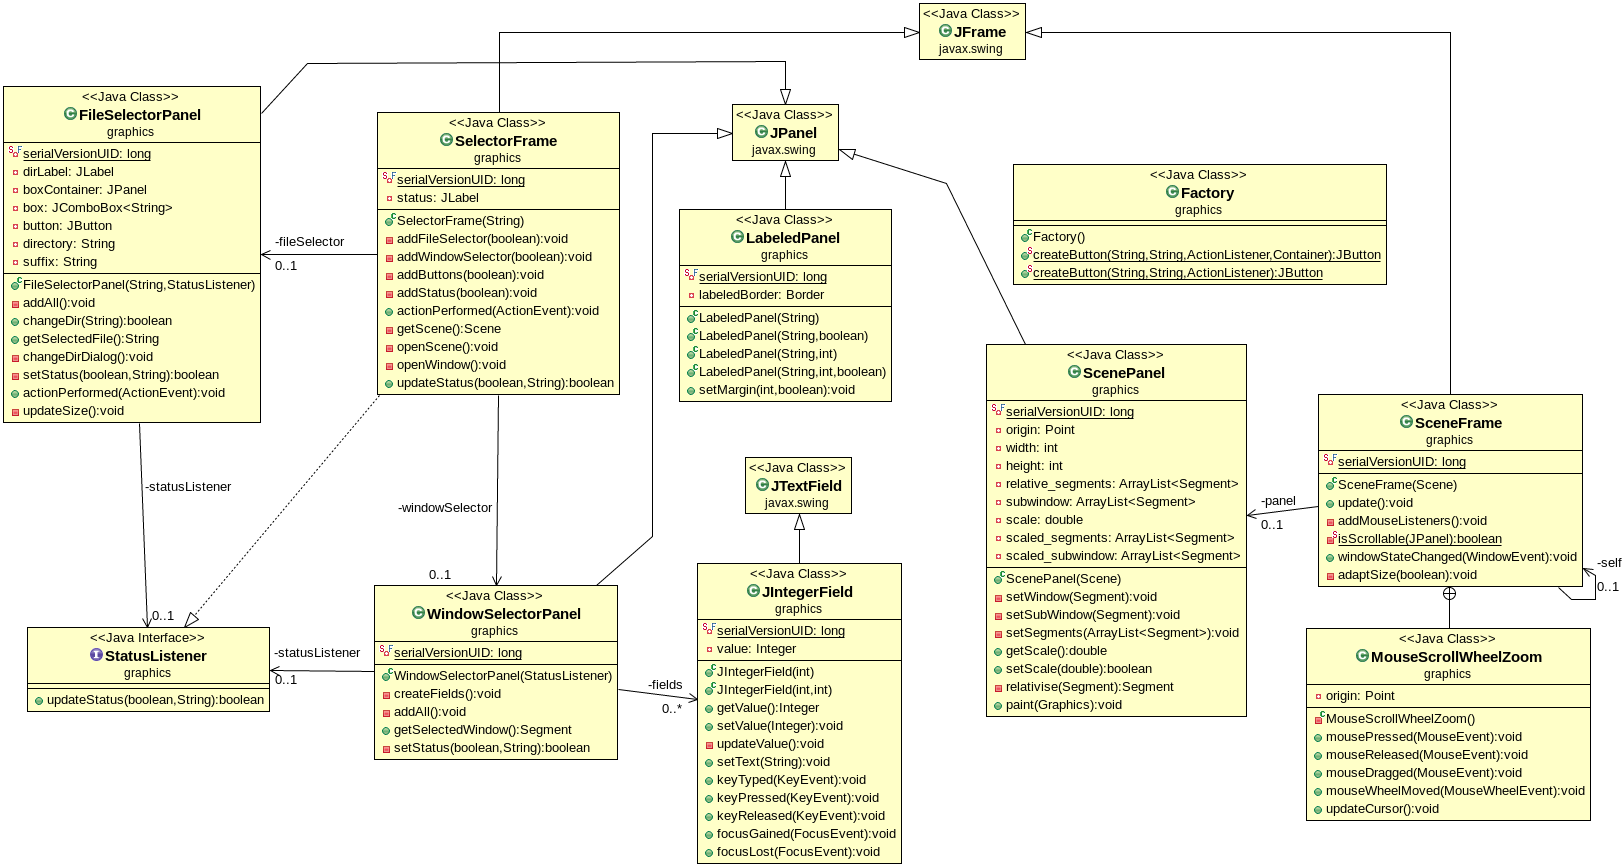
\includegraphics[scale=0.25]{../src/UML/graphics.png}

\subsection{Pst et BasicPst}
BasicPst correspond au PST gérant efficacement une fenêtre de type $[-\infty, X']$ x $[Y, Y']$. Afin de gérer toutes les transformations, nous avons créé une autre classe Pst qui comporte 4 BasicPst avec :
\begin{enumerate}
	\item les segments originaux pour les fenêtres $[-\infty, X']$ x $[Y, Y']$ ;
	\item les segments échangés pour les fenêtres $[X, X']$ x $[-\infty, Y']$ ;
	\item les segments opposés pour les fenêtres $[X, +\infty]$ x $[Y, Y']$ ;
	\item les segments échangés et opposés pour les fenêtres $[X, X']$ x $[Y, +\infty]$ ;
\end{enumerate}

Cette classe s'occupe de choisir l'arbre sur lequel effectuer le windowing afin d'obtenir la meilleure efficacité. Plusieurs arbres sont utilisés pour les fenêtres $[X, X']$ x $[Y, Y']$.

\newpage
\section{Algorithmes et explications}
Dans cette section, nous exposons nos différents algorithmes importants en pseudo-code ainsi que leur complexité en temps. Une courte explication en français y est aussi ajoutée afin de favoriser la compréhension de ceux-ci et leurs utilisations.

\subsection{Hauteur de l'arbre}
Afin de compléter les différentes explications, nous allons en premier lieu vous expliquer et prouver que la hauteur de l'arbre est en $\mathcal{O} ( log_2(n) ) $ où n est le nombre de segments présents dans le plan. En effet, la structure du Pst adapté est un arbre complètement équilibré, nous pouvons donc comparer celui-ci à un AVL dont la balance de chaque nœud en valeur absolue ne dépasse pas 1.
Nous avons effectué un test dans notre classe PstTests dans notre projet visant à vérifier ceci. L'intuition de cet équilibre s'explique par le fait que lors de la construction de l’arbre, pour chaque nœud de l'arbre, nous répartissons le nombre de segments restants en deux parties égales à un segment près, et chaque partie constitue toutes les données du sous-arbre gauche ou droit de ce nœud.

\subsection{Construction de l'arbre}

\subsubsection{Algorithmes}

\begin{algorithm}
\caption{Construction de l'arbre}
\begin{algorithmic}[1]
\REQUIRE une liste de Segment $A$, un PstNode $Root$ qui est la racine de l'arbre 
\ENSURE /
\STATE $A \leftarrow heapSort(A)$
\STATE $root \leftarrow makePstNode(A) $
\end{algorithmic}
\end{algorithm}

\begin{algorithm}
\caption{makePstNode}
\begin{algorithmic}[1]
\REQUIRE une liste de Segment triée en y $A$ 
\ENSURE un PstNode qui représente la racine de l'arbre
\IF{$A$ est vide}
\RETURN $null$
\ENDIF
\STATE $node \leftarrow A[getMinX()] $
\IF{$A$ est non vide}
\STATE $i \leftarrow longueur(A)/2$
\STATE $node.median \leftarrow A[i].y1 $
\STATE $node.left \leftarrow construct(A.sousListe(0,i)) $
\STATE $node.right \leftarrow construct(A.sousListe(i,longueur(A))) $
\ENDIF
\RETURN node
\end{algorithmic}
\end{algorithm}

\newpage
\begin{algorithm}
\caption{getMinX}
\begin{algorithmic}[1]
\REQUIRE une liste de Segment $L$
\ENSURE l'indice entier de l’élément minimum en X
\IF{$L$ est vide}
\RETURN -1
\ENDIF
\STATE $min \leftarrow 0$
\FOR{$i \leftarrow 1$ à $longueur[A]$}
\IF{$A[i].minX() < A[min].minX() $}
\STATE $min \leftarrow i$
\ENDIF
\ENDFOR
\RETURN $min$
\end{algorithmic}
\end{algorithm}

\subsubsection{Explication}

Nous construisons ici l'arbre de haut en bas, ayant initialement la racine qui est le minimum en x des segments, nous effectuons ensuite une séparation des données en deux par rapport à la médiane, qui est la valeur en y1 (minimum en y du segment) se trouvant au milieu de la liste, et ceci récursivement.

Nous séparons ainsi à chaque étape la liste des segments en deux parties égales en taille à une valeur près, que nous répartissons entre les deux fils (première moitié au fils gauche et deuxième moitié au fils droit). Bien sûr pour que ceci soit possible, nous avons trié les segments par ordre croissant suivant leur composante en y1 avant d'utiliser la liste pour la création de l'arbre.

\subsubsection{Complexité dans le pire des cas}
Nous commençons d'abord par calculer la complexité dans le pire des cas en temps de l'algorithme 3.
Les 4 premières lignes sont en $\mathcal{O} (1)$, ainsi que les lignes 7 et 10, car le retour est constant, la condition du if est constante et une affectation de valeur est constante en temps. La condition du if de la ligne 6 est elle aussi constante, car nous faisons une comparaison de valeurs (temps constant) et qu'avoir accès à la valeur du minimum x d'un segment se fait en temps constant aussi (minX() ).

Nous avons donc un for en ligne 5 qui est en $\mathcal{O}(n)$ où n est la taille de la liste.
L'algorithme possède donc une complexité de $\mathcal{O}(n)$ au total.
\\
En ce qui concerne l'algorithme 2, les lignes s'exécutent toutes en temps constant pour les mêmes raisons que celles énoncées pour le $3^e$ algorithme exceptées les lignes 4,7 et 8.
En effet, la ligne 4 s’exécute en $\mathcal{O}(n)$ où n est la taille de la liste donnée en paramètre, par la preuve ci-dessus. Nous effectuons ensuite deux appels récursifs aux lignes 7 et 8, ce qui nous donnera une complexité finale de l'algorithme en temps de $\mathcal{O}(n.log(n))$. Voici le raisonnement pour trouver cette complexité finale :

Notre algorithme s'effectue à chaque étape de la récursivité en $\mathcal{O}(n)$ dû à la recherche du minimum dans la liste. Nous effectuons ensuite un appel récursif sur une moitié de liste, et un autre appel sur l'autre moitié.\\ Ce qui nous donne donc une complexité de $\mathcal{O}(n)$ + $\mathcal{O}(n/2)$ + $\mathcal{O}(n/2)$ + $\mathcal{O}$(de la prochaine étape de la récursivité) + ...\\Ce qui nous donne donc une complexité de $\mathcal{O}(n)$ + $\mathcal{O}(n)$ + $\mathcal{O}$(de la prochaine étape) + ...\\ On voit donc qu'à chaque niveau de l'arbre, nous effectuons des calculs en $\mathcal{O}(n)$, nous les effectuons log(n) fois qui est la hauteur de l'arbre. Nous aurons donc une complexité finale de l’algorithme 2 en $\mathcal{O}(n.log(n))$ où n est la taille de la liste initialement donnée en paramètre à la fonction.
\\

Finalement, en ce qui concerne l'algorithme 1, celui-ci possède une première ligne en $\mathcal{O}(n)$ (complexité en temps du heapSort, notion étudiée au cours), et une seconde en $\mathcal{O}(n.log(n))$. Nous aurons donc une complexité finale de $\mathcal{O}(n.log(n))$

\subsection{Windowing}


\subsubsection{Algorithmes}

\begin{algorithm}
\caption{Windowing}
\begin{algorithmic}[1]
\REQUIRE un Segment $window$ représentant la fenêtre à appliquer
\ENSURE Une liste contenant tous les Segments dans la fenêtre
\RETURN window2($window$,$true$,$true$)
\end{algorithmic}
\end{algorithm}

\begin{algorithm}
\caption{Windowing2}
\begin{algorithmic}[1]
\REQUIRE un Segment $window$(objet) représentant la fenêtre à appliquer, un booléen $down$ et un booléen $center$ représentant les type de report à appliquer
\ENSURE Une liste contenant tous les Segments dans la fenêtre
\STATE $window \leftarrow window.getWindow()$
\STATE $reported \leftarrow$ nouvelle liste vide
\STATE subwindow($root$,$window$,$reported$,$true$,$true$)
\RETURN $reported$
\end{algorithmic}
\end{algorithm}

\newpage

\begin{algorithm}
\caption{Subwindowing}
\begin{algorithmic}[1]
\REQUIRE un Node $node$, un Segment $window$, une liste de Segment $reported$, un booléen $down$ et un booléen $center$
\ENSURE / Mais effet de bord : $reported$ contient tous les Segments dans la fenêtre
\IF{$node$ est vide}
\STATE fin de l'algorithme
\ENDIF
\STATE $S \leftarrow node.getSegment()$
\IF{$center$ est faux et $S.minX()>window.x1$}
\STATE fin de l'algorithme
\ENDIF
\IF{$S.minX()>window.x2$}
\STATE fin de l'algorithme
\ENDIF


\IF{$center$ est vrai et $reportCenter(S,window)$ est vrai}
\STATE Ajout de $S$ dans $reported$
\ENDIF
\IF{$down$ est vrai et $reportDown(S,window)$ est vrai}
\STATE Ajout de $S$ dans $reported$
\ENDIF
\IF{$reportLeft(S,window)$ est vrai}
\STATE Ajout de $S$ dans $reported$
\ENDIF

\IF{$down$ est vrai ou $node.median >= window.y1$}
\STATE subWindowing($node.left,window,reported,down,center)$
\ENDIF

\IF{$node.median <= window.y2$}
\STATE subWindowing($node.right,window,reported,down,center)$
\ENDIF

\end{algorithmic}
\end{algorithm}


\subsubsection{Explication}

Le windowing appliqué dans les algorithmes ci-dessus est basé sur un windowing d'une fenêtre de type : \begin{itemize}
\item soit $[-\infty;x2]X[y1;y2]$,
\item soit $[x1;x2]X[y1;y2]$.
\end{itemize}
Selon cette hypothèse, nous avons considéré tous les cas de segments devant être considérés dans la fenêtre (au moins un point dans la fenêtre ou passant au travers) et ceux qui ne devaient pas s'y trouver. Afin de favoriser la compréhension de notre algorithme, nous expliquons les deux algorithmes l'un après l'autre.

En ce qui concerne le windowing (algorithme 4), il ne nécessite pas d'explication supplémentaire, le pseudo-code est très clair.

Pour l'algorithme 5 (windowing2), l'algorithme effectue dans cet ordre ces différentes actions : rendre la structure représentant la fenêtre ordonnée(x1<x2 et y1<y2) afin de respecter la notion mathématique d'une fenêtre et simplifier le code, et ensuite calculer à l'aide de l'algorithme 6 les segments dans la fenêtre pour pouvoir les retourner dans une liste.

L'algorithme 6 est la partie plus délicate de l'algorithme. En effet, c'est ici que nous avons mis en œuvre l'exploration de l'arbre pour prendre tous les segments qui nous intéressent. Nous avons donc procédé à une série de vérifications de conditions.

Tout d'abord, nous vérifions que le nœud n'est pas vide (cas se produisant après l'exploration d'une feuille).

Pour les deux conditions suivantes, nous cherchons les conditions d'arrêt de l'algorithme qui pourraient se produire avant d'arriver à la fin de l'arbre.

La première condition vérifie que nous ne devons plus prendre de segments se trouvant à l'intérieur de la fenêtre et que le nœud courant dans lequel nous nous trouvons se trouve soit dans la fenêtre, soit à droite de la fenêtre pour ses coordonnées en x. Par définition de la structure, nous savons donc que tous les nœuds fils se trouvent soit dans la fenêtre, soit à droite de la fenêtre en x (car le nœud courant est le minimum en x). Nous pouvons donc arrêter l'algorithme et ignorer ses descendants.

La deuxième condition d'arrêt est le cas où le segment du nœud courant se trouve complètement à droite de la fenêtre en x, nous pouvons donc l'ignorer et ignorer les sous-arbres qui suivent car ils seront tous à droite de la fenêtre (donc pas dedans) par la définition de la structure comme ci-dessus. Dis autrement, les coordonnées en x du segment se trouvant dans le nœud courant nous indiquent qu'elles sont strictement plus grandes que la fenêtre, or ce segment possède la coordonnée en x minimum du sous-arbre dans lequel elle se trouve, il faut donc ignorer ses descendants.

En ce qui concerne les 3 conditions suivantes dans l'algorithme, celles-ci sont utilisées pour détecter quels segments se trouvent réellement dans la fenêtre, cette détection est faite durant toute l'exploration de l'algorithme dans l'arbre. Les conditions booléenne $down$ et $center$ sont utilisées afin de savoir quel type de report nous devons effectuer. En effet nous devons pouvoir détecter les différents types de segments énoncés lors de l'explication du windowing dans le point précédent "Pst adapté".

Nous appelons donc trois méthodes qui testent ces différentes conditions. Nous n'avons pas fourni les pseudo-codes correspondant à ces méthodes qui effectuent simplement une condition et un retour booléen décrivant si le segment est à prendre en compte ou pas. Nous avons favorisé une explication écrite plutôt qu'algorithmique ce qui est plus compréhensible pour le lecteur et moins fastidieux à lire. Bien sûr pour plus de détails, le code source est disponible vous donnant un exemple pratique d'appliquer les différents reports.

Les différentes conditions de reports sont donc celles-ci :\begin{itemize}
\item[\textbf{reportCenter()}] Pour détecter les segments ayant leur point de départ dans la fenêtre.

\item[\textbf{reportDown()}] Pour détecter les segments verticaux ayant leur point de départ en dessous de la fenêtre et passant à travers la borne inférieure de la fenêtre.

\item[\textbf{reportLeft()}] Pour détecter les segments horizontaux ayant leur point de départ à gauche de la fenêtre et passant à travers la borne gauche de la fenêtre.

\end{itemize}
Nous avons ainsi géré tous les segments visibles dans nos deux types de fenêtre.

Finalement nous regardons par rapport à la médiane du nœud courant où nous devons nous déplacer dans l'arbre. Nous considérons donc les deux limites en y de la fenêtre pour savoir quand se déplacer à gauche dans l'arbre (éléments <= à la médiane en y1) ou à droite (éléments >= à la médiane en y1). Nous faisons donc des appels récursifs pour avancer toujours dans la bonne direction dans l'arbre et éviter des reports inutiles.

\subsubsection{Complexité dans le pire des cas}

Les différentes lignes dans les algorithmes 4 et 5 sont tous en $\mathcal{O}(1)$ car nous ne faisons que des appels à des fonctions, des retours de valeur et un appel à getWindow() dans l'algorithme 5-ligne 1, qui s'effectue aussi en $\mathcal{O}(1)$ aussi car il ne fait que donner un nouveau segment en prenant les données du premier. Le coût du windowing sera donc dû à l’exécution de la fonction subwindowing() qui va effectuer le réel travail d'exploration dans le Pst.

Nous calculons donc la complexité en temps de l'algorithme 6.
Pour les lignes 1 à 10, elles s’exécutent toutes en $\mathcal{O}(1)$ car nous faisons de simples tests booléens sur des valeurs, des accès à des variables d'objets, une affectation à une variable, et le corps de toutes les conditions est en $\mathcal{O}(1)$ aussi.
Pour les lignes 11 à 19, les différents tests booléens s'effectuent en $\mathcal{O}(1)$, ainsi que l'ajout à une liste et l'appel aux différents reports. En effet ceux-ci testent juste des conditions sur les coordonnées d'après les cas et retournent un booléen, elles s’exécutent donc en un temps constant également.

Il nous reste donc les lignes 20 à 24. En ce qui concerne ces lignes, l'étude de leur complexité est plus particulière. En effet elles effectuent un appel récursif selon certaines conditions qui ont un coût en temps de $\mathcal{O}(1)$.
Considérant que l'algorithme est jusqu'ici en $\mathcal{O}(1)$, l'algorithme se réalisera en $\mathcal{O}(1)$ x le nombre d'appels récursifs.

Si nous analysons les appels nous constatons que les appels récursifs peuvent se réaliser soit sur le sous-arbre gauche du nœud courant (initialement la racine) si la fenêtre se trouve totalement à gauche de la médiane, soit le sous-arbre droit si la fenêtre se trouve totalement à droite de la médiane, soit les deux sous-arbres si la médiane se trouve dans la fenêtre. Nous remarquons aussi qu'à chaque avancement dans l'arbre, la médiane du nouveau nœud courant diminue(fils gauche) ou augmente (fils droit) par rapport à son père.

Le pire cas est certainement celui où tous les segments sont dans la fenêtre. Dans ce cas, il faut parcourir tous les nœuds et la complexité de notre algorithme est en $\mathcal{O}(n)$.

\subsection{Modification des fenêtres}

\subsubsection{Explication}
Le but de cette classe est de créer différents Pst en changeant les coordonnées des segments afin de transformer n'importe quel type de fenêtre lors du windowing en notre fenêtre idéale. Nous ne réexpliquons pas tout le principe en détail, car il a déjà été expliquer précédemment dans le rapport.

Nous créons donc 4 listes avec les segments changés afin de construire 4 Pst différents sur lesquels nous appliquerons nos différents windowing. Nous réutiliserons la même méthode à la fin d'un windowing pour avoir les segments d'origine.

\subsubsection{Complexité dans le pire des cas}
Deux calculs de complexité en temps doivent être pris en compte :
\begin{itemize}
\item Les transformations de segments, qui se font en $\mathcal{O}(n)$ chacune. Nous additionnons donc 4 fois cette complexité, ce qui nous donne du $\mathcal{O}(n)$

\item Les constructions des 4 arbres , qui se font chacune en $\mathcal{O}(n.log(n))$, ce qui nous donne aussi un total de $\mathcal{O}(n.log(n))$.

\end{itemize}

Notre complexité finale pour la construction généralisée sera donc en $\mathcal{O}(n.log(n))$ dans le pire des cas.

\newpage
\section{Mode d'emploi}
Pour lancer une commande, rendez-vous dans le dossier racine du projet à l'aide du terminal.

\subsection{Javadoc}
Pour compiler la Javadoc, entrez la commande \colorbox{lightgray}{ant javadoc}. La documentation compilée se trouve alors dans le répertoire \textbf{build/doc/}.

\subsection{Tests unitaires}
Pour lancer les tests unitaires, entrez la commande \colorbox{lightgray}{ant test}.

\subsection{Lancement du programme}
Pour compiler et lancer le programme à partir des fichiers sources, entrez la commande \colorbox{lightgray}{ant run}.

\subsection{Interface utilisateur}
L'interface utilisateur est particulièrement intuitive et ressemble à ceci :

\centerline{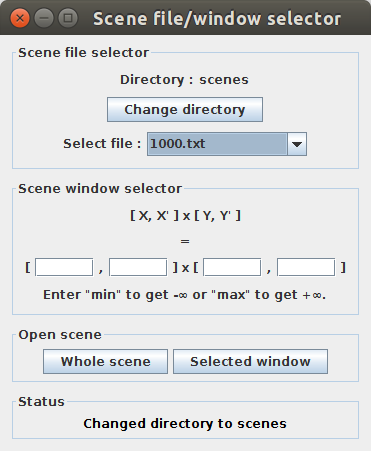
\includegraphics[scale=0.5]{images/ui.png}}

Comme vous pouvez le voir, l'interface est divisée en 4 parties :
\subsubsection{Sélecteur de fichier}
La première partie contient un sélecteur de fichier qui vous proposera par défaut de choisir un fichier .txt parmi ceux présents dans le dossier \textbf{scenes} (relatif à l'application). Vous pouvez changer de répertoire si vous souhaitez choisir des fichiers qui se trouvent à un autre emplacement.

\subsubsection{Sélecteur de fenêtre}
La seconde partie vous permet d'indiquer au programme la fenêtre à utiliser pour effectuer le windowing. Entrez "min" et "max" pour indiquer respectivement $-\infty$ et $+\infty$.

\subsubsection{Ouvreur de scène}
La troisième partie vous propose deux boutons. L'un ouvrira, dans une nouvelle fenêtre, toute la scène contenue dans le fichier sélectionné par le sélecteur de fichier. Exemple :

\centerline{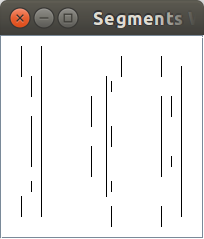
\includegraphics[scale=0.5]{images/ui_whole_scene.png}}

L'autre bouton ouvrira, également dans une nouvelle fenêtre, la scène contenue dans le fichier sélectionné, après y avoir appliqué le windowing en utilisant la fenêtre fournie par le sélecteur de fenêtre. La fenêtre sélectionnée s'affichera en rouge par dessus la scène. Exemple :

\centerline{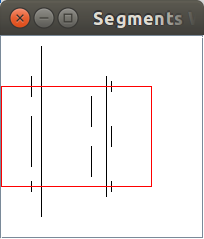
\includegraphics[scale=0.5]{images/ui_restricted_window.png}}

Si la scène est trop grande pour entrer dans la fenêtre de visualisation nouvellement ouverte, des barres de défilement apparaîtront et il vous sera possible de naviguer dans la scène en maintenant le pointeur de la souris enfoncé.

Si vous le désirez, il est possible de changer la taille de la visualisation à l'aide de la molette de votre souris.

\subsubsection{Information sur l'état du programme}
La quatrième et dernière partie de l'interface affiche l'état du programme. Les erreurs y sont affichées en rouge, alors que les informations y sont en noir.

\section{Illustrations}
Cette section sert d'illustration, afin de vous permettre d'observer différents cas d'application du windowing via l'application que nous avons créée.
Cette image concerne des applications du windowing sur des segments horizontaux:

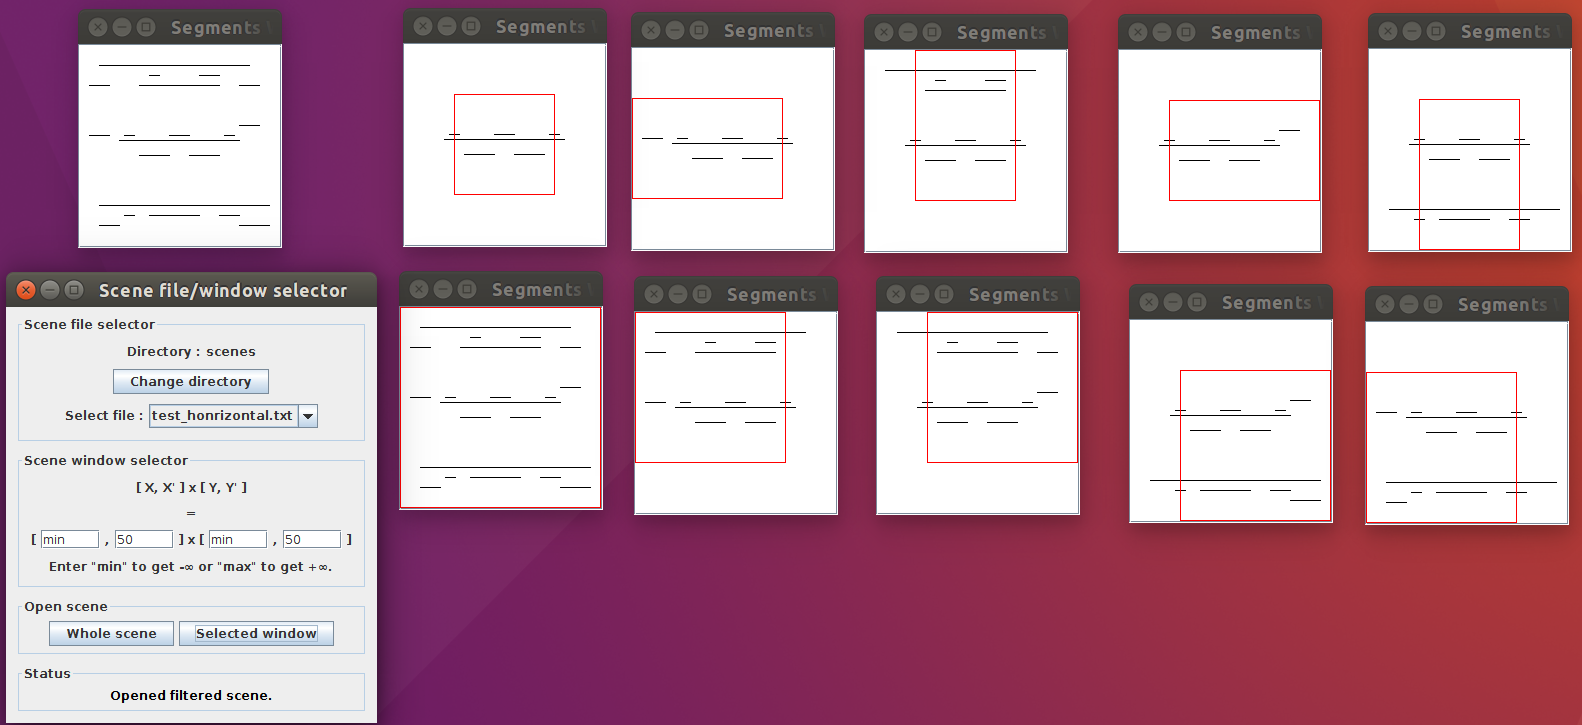
\includegraphics[scale=0.25]{images/test_horizontal.png}

Cette image concerne des applications du windowing sur des segments verticaux:

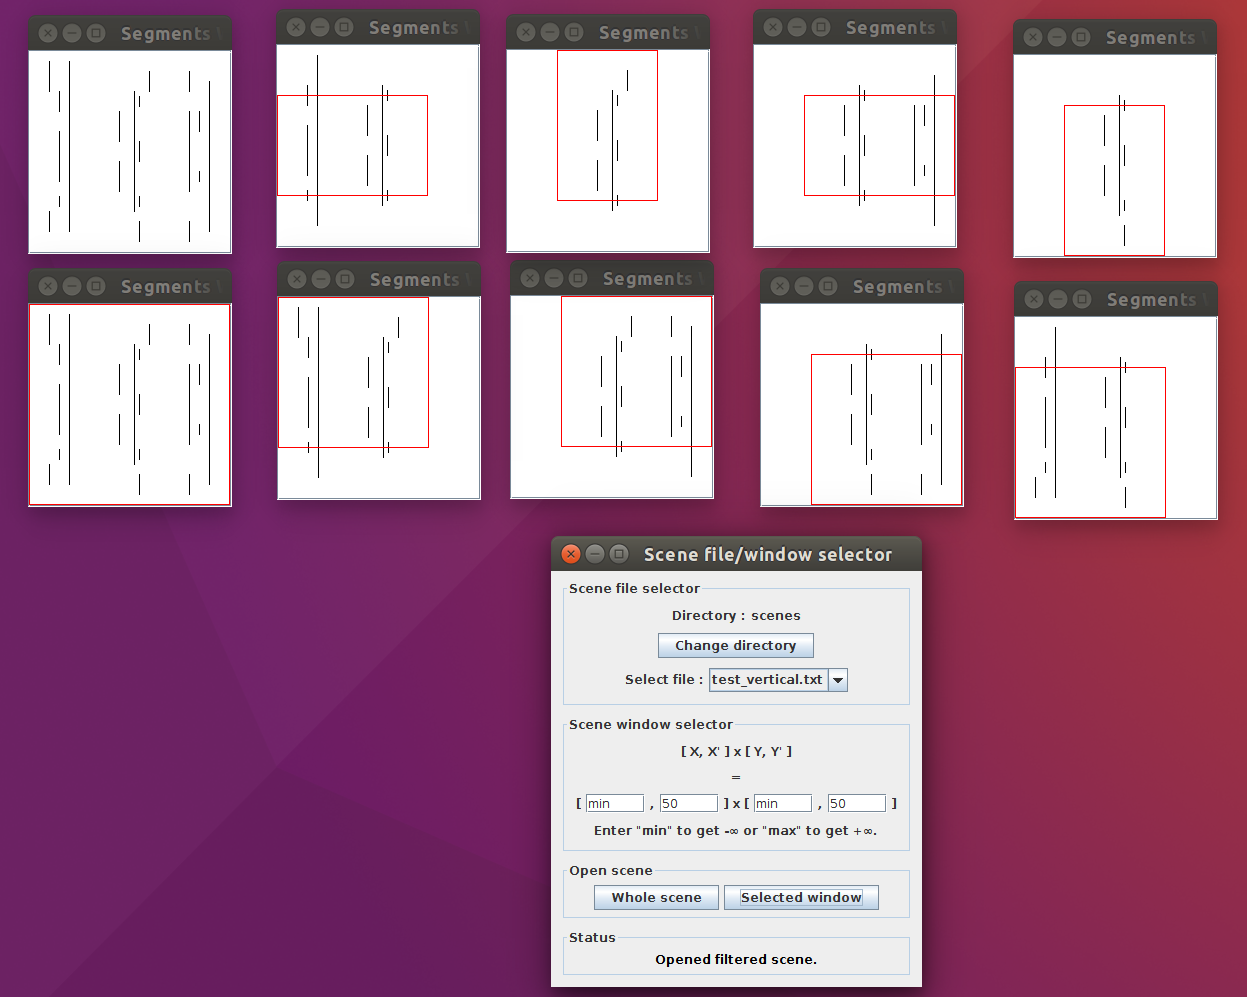
\includegraphics[scale=0.25]{images/test_vertical.png}

\section{Améliorations possibles}
Plusieurs améliorations auraient encore été possibles :
\begin{itemize}
	\item calculer le point moyen (parmi tous les points définissant les segments) et décider des transformations à utiliser en fonction de la situation de la fenêtre fermée par rapport au point moyen ;
	\item bien qu'il ne nous ait pas été demandé de traiter les fenêtres ayant 2 bornes infinies, décider des transformations à utiliser en fonction de l'orientation des 2 bornes.
\end{itemize}

\section{Conclusion}
Nous avons bien réalisé les objectifs fixés dans l'introduction, à savoir créer et manipuler une structure de données non vue au cours. Pour ce faire, nous avons utilisé différents concepts vus au cours "Structure de données 2", comme les tas et les ABR.

Ce travail nous a permis de faire un peu de "recherche" en groupe, dans l'optique de résoudre un problème nouveau. Lors de nos réunions de groupe, nous avons pu partager nos points de vue individuels et ainsi considérer le problème sous différents aspects. Nous gardons un souvenir très positif de ce travail. Nous tenons à remercier les professeur et assistant qui nous ont soutenues pour mener à bien ce projet, à savoir BRUYÈRE Véronique et DEVILLEZ Gauvain.


\end{document}